\chapter{Design}

Designing this system could take two different paths in order to create a directory tree representing the database. The first is to have a program look for changes in both the database and filesystem and then mirrors the changes from each to the other. The second method is to write a filesystem that is constantly being called with callbacks when the user performs an action such as creating a folder or deleting a file.

\section{Polling or Filesystem?}

\subsection{Polling}

This program would then be run at regular intervals to give the illusion that they were directly linked. There are numerous problems with this implementation with the most prominent being detecting the changes made on each side. Not all database management systems allow for the placement of triggers or streaming of incoming data to another source. The other side is simpler as there are already methods of looking for updated files in the form of modification dates and operating system APIs for registering for callbacks of changes such as \texttt{inotify} for Linux and \texttt{fs-events} for Mac OS X.

This is a less than ideal method of scanning for updates when we may have millions of records and therefore millions files that need checking. This solution just does not scale well even with the operating system assistance. Additionally, the constant polling of the filesystem is a lot of wasted work that will deplete the battery of laptops unnecessarily and waste power on desktop machines. Instead, we should flip the problem around and instead of looking for the files that have been changed, we should get any file that changes to tell us about itself.

\subsection{Filesystem}

By using a filesystem instead of an separate polling program we tighten the feedback loop from changes to the files to the database. By doing this we avoid the potentially expensive operations of scanning the filesystem for changes and have direct callbacks that reference the exact file changed. This has the additional advantage of automatically handling migrating any changes back from the database to the filesystem just by refreshing the view.

\section{Scaling Issues}

There is some concern about how this will scale up to the sizes that databases can reach. There are some unknowns such as how a filesystem will perform once it has millions of files in it, each representing a record in the database. Since users demand that a filesystem is responsive then a non-functional requirement should be made that the database returns all queries in a responsive manner. There are numerous ways that this could be done such as simple caching of values outside the database all the way up to using previous usage patterns to scan across the data on the disk in order to load it into memory before the query is ever made to creating useful indexes automatically to help regularly slow queries. However, it is unwise to spend unnecessary time considering solutions to problems that may not occur.

\section{The Querying Problem}

A database has 3 main duties when it comes to presenting the user with data: querying, updating and deleting. Our current solution to the problem provides a good solution to updating and deleting records but querying the database beyond basic operations is not easy to do with the limited actions available to the filesystem.

In order to allow the user to perform more complex queries on the database a separate application is needed. However it is critical that still presents the database as a filesystem. If we look at how users perform complex sequences of operations on a filesystem currently then there are two different approaches depending on the level of expertise of the user.

\subsection{Mirroring Filesystem Solutions}

If we have a task that we would like to perform such as resizing all of the images in a folder that were taken in the last week and which have ``flower'' in the filename then depending on the level of expertise of the user then they will probably approach it in two different ways.

A technical user will probably write a shell script or use multiple commands piped together to achieve the intended effect. A command such as the following will perform the task shown in figure \ref{fig:shell}.

\begin{figure}[ht!]
  \centering
	\begin{verbatim}
	  find . -type f -name ".jpg" |
	    grep "flower" |
	    xargs convert -resize 50%
	\end{verbatim}
  \caption{Shell Workflow}
  \label{fig:shell}
\end{figure}


Instead of performing the action in one step the user splits up the command into 3 logical steps of find the pictures, filter the ones with flower in the name, and finally perform the resizing.

A non-technical user has a number of available operations to them. The most widely used among Macintosh users is probably a program called Automator which is bundled with the operating system. It allows the user to do a similar thing to shell scripts by composing a workflow of similar duties to the programs above.

\begin{figure}[ht!]
  \centering
  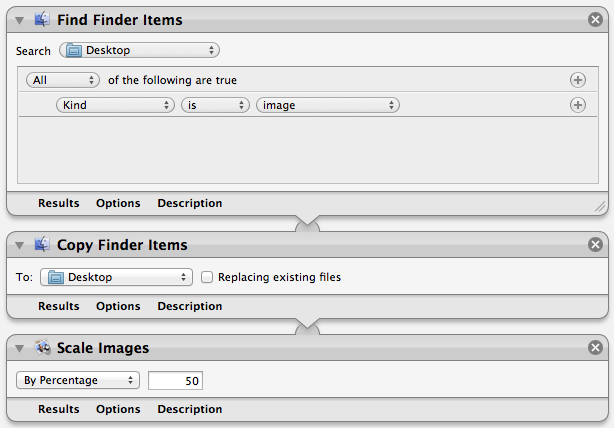
\includegraphics[width=0.9\textwidth]{images/automator}
  \caption{Automator Workflow}
  \label{fig:automator}
\end{figure}

We should be able to take this existing solution and paradigm and apply it to the database querying problem. I believe that this will work specially well if we make the records maintain their file-like qualities even inside the application.

In order to convert this graph of command into a database action we are going to need to generate \ac{SQL} which will perform the desired action. This is the next design challenge.

\section{Creating SQL}

The task of creating \ac{SQL} has been solved many different times when creating \acp{ORM}. These often use Relational Algebra or something similar to it to represent the compounded operators before being converted to a sensible SQL statement. Using a similar approach for this task would be sensible as it mimics the graph structure that is described above. For example, a filter node in the application above is equivalent to a selection wrapping everything above it in the graph.

This intermediate relational algebra representation also has the advantage of completing the metaphor above by replacing the more technical users requirement of being able to drop down to a more direct interface to controlling the database.

To this end I'm going to create an intermediate language that allows the user to create complex \ac{SQL} queries by writing relational algebra in an imperative style. This can then be combined with the filesystem by allowing these files to be saved on it and having it return the results.